\documentclass[11pt]{article}
\usepackage{amsmath}
\usepackage{amsfonts}                                                                                                                                                      
\usepackage{graphicsx}
\usepackage{hyperref}
\tolerance=1
\emergencystretch=\maxdimen
\hyphenpenalty=10000
\hbadness=10000
                                        
\begin{document}
\begin{sloppypar}
\title{Theorems in Complex Analysis}
\author{A cheat sheet for formulae \\Anurag Pallaprolu\\ BITS Pilani}
\maketitle
\tableofcontents
\setcounter{tocdepth}{3}
\clearpage
\section{Preliminary Definitions and Formalities}
We shall start with the basics of the complex number field $\mathbb{C}$. The axiomatic definition follows from the fact that they are all ordered pairs of two reals plotted on the Argand diagram. To name a few standard field properties

\begin{enumerate}

\item $z_{1} + z_{2} = z_{2} + z_{1}$

\item $(z_{1} + z_{2} )+ z_{3} = z_{1} + (z_{2}+z_{3})$
\item $z + 0 = z$
\item $z*1 = z$

\end{enumerate}

Now we move on to a few standard inequalities like the two triangle inequalities:

\begin{description}
\item[Triangle Inequality] \hfill \\
	$|z_{1}\pm z_{2}| \leq |z_{1}|+|z_{2}|$ \\
	$|z_{1}\pm z_{2}| \geq ||z_{1}|-|z_{2}||$ \\
	We can generalize the first one by induction\\
	\begin{equation}
	|\sum_{i=1}^{n} z_i| \leq \sum_{i=1}^{n} |z_i|
	\end{equation}
\end{description}

Also we must not forget the most important equation of all of complex analysis, the Euler equation and its obvious generalization, the De Moivre formula

\begin{equation}
	\tag{*}
	\exp(i\theta) = \cos(\theta) + i\sin(\theta)
	\label{eqn:Euler}
\end{equation}
\begin{equation}
	\exp(in\theta) = \cos(n\theta) + i\sin(n\theta)
\end{equation}

The nth roots of any complex number z can be given from the above forumlae as
\begin{equation}
	z = \sqrt[n]{r_{0}} exp(i(\theta+2k\pi)/n)
\end{equation}
where $r_{0}$ is the length or the modulus of z and $\theta$ is the argument of z in the complex plane. This will be all for the basic equations that one must have in mind when studying complex analysis. 

\section{Analytic Functions}
Functions of a complex variable share many properties similar to vector fields. To review the definition of a vector field, it is a vector function whose components are also functions of the cartesian or any set of coordinates. Mathematically, we can state a vector field $\mathcal{F}: \mathbb{R}^{3} \rightarrow \mathcal{V}$ as,
$$\mathcal{F}(x,y,z) = u(x,y,z)\mathbf{i} + v(x,y,z)\mathbf{j} + w(x,y,z)\mathbf{k}$$
except that in the case of complex numbers, we usually map from the set of real ordered pairs to the complex number space as 
$$f(z) = u(x,y)+iv(x,y)$$ where both $u$ and $v$ are functions from $\mathbb{R}^{2} \to \mathbb{R}$. Most of the functions that occur in complex analysis starkly differ from what we encounter in reals that is, they are mostly multivalued, even standard single valued functions like the logarithm. 

\subsection{Limits and continuity}
As in any analysis course, we have to first focus on limits and continuity. Limits of complex functions are rather simple to evaluate, following similar rules as to real functions. Here are two theorems that should suffice the discussion on limits.
\begin{description}
\item[Theroem 1] \hfill \\
	If $f(z) =  u(x,y)+iv(x,y)$ and $z_{0} = x_{0}+iy_{0}$ and $w_{0} = u_{0} + iv_{0}$., then if 
	$$lim_{z \to z_{0}} f(z) = w_{0}$$ iff
	$$lim_{(x,y) \to (x_{0},y_{0})} u(x,y) = u_{0}$$ $$lim_{(x,y) \to (x_{0},y_{0})} v(x,y) = v_{0}$$
\item[Theorem 2] \hfill \\
	Suppose that $lim_{z \to z_{0}} f(z) = w_{0}$ and $lim_{z \to z_{0}} F(z) = W_{0}$ then
	$$lim_{z \to z_{0}} f(z) + F(z) = w_{0} + W_{0}$$
	$$lim_{z \to z_{0}} f(z)*F(z) = w_{0}*W_{0}$$
	$$lim_{z \to z_{0}} f(z)/F(z) = w_{0}/W_{0}$$
The last equality will exist under obvious circumstances. 
\end{description}

So much for limit evaluation. Let us now look at continuity of functions. This is too, much similar to what we have studied in real analysis. To be more succint, a function f(z) is continuous at $z_{0}$ if the following conditions are satisfied:\\
$$lim_{z \to z_{0}}f(z)$$ exists\\
$$f(z_{0})$$ exists \\
$$lim_{z \to z_{0}}f(z) = f(z_{0})$$ \\
And as usual, there is the all the more important theorem of continuity
\begin{description}
\item[The composition of continuous functions is itself a continuous function]  \hfill \\
	A statement which can be proven directly from the Cauchy definition of continuity. 
\item[Continuity at a point and the value of the function] \hfill \\
	If a function is continuous and non zero at a point, then it is also non zero in any $\delta$ interval of the point. Failure of this clause might lead to pathological properties of functions at hand such as fractal discontinuities etc.
\end{description}

\subsection{Derivatives and Analytic Property}
Now, we get to the interesting part of analysis. The definition of the complex derivative is given below
$$f\rq{}(z_{0}) = lim_{z \to z_{0}}\frac{f(z) - f(z_{0})}{z-z_{0}}$$. Functions of the explicit complex variable z, the calculus of such functions is not complicated as all that is needed is to replace z as any real quantity and proceed with the analysis. However, functions of two $real$ variables, we have to be careful, for they are restricted by the concept of $analyticity$.
But first, the important theorem
\begin{description}
\item[Cauchy Riemann Equations] \hfill \\
	If the function $$f(z)= u(x,y)+iv(x,y)$$ is differentiable at any point z, then the components u and v should satisfy the Cauchy Riemann conditions i.e;
	\begin{equation}
	\partial u/\partial x = \partial v/\partial y
	\end{equation}
	\begin{equation}
	\partial u/\partial y = -\partial v/\partial x
\end{equation}
\end{description}
 The Cauchy Riemann conditions are neccesary but not sufficient conditions for differentiability. That is, a slight adjustment can be made so that these equations provide a sufficient condition. The theorem below follows,
 \begin{description}
\item[Modified Cauchy Riemann Theorem] \hfill \\
	If the function $$f(z)= u(x,y)+iv(x,y)$$ is differentiable at any point z, and is defined through an $\delta$ neighbourhood of a point z and the first order partial derivatives of u and v exist everywhere in the neighbourhood. If the partials are smooth enough, and satisfy 
	$$\partial u/\partial x = \partial v/\partial y$$
	$$\partial u/\partial y = -\partial v/\partial x$$
then the hypothesis is claimed to be true. 
\end{description}
Now we can extend the equations to polar coordinates as well. Noting that there is \eqref{eqn:Euler} for switching from both systems, we can see that the new equations take the form of,
	\begin{equation}
	r\partial u/\partial r = \partial v/\partial \theta
	\end{equation}
	\begin{equation}
	\partial u/\partial \theta = -r\partial v/\partial r
\end{equation}
\begin{description}
\item[Harmonic Functions] \hfill \\
	Functions which satisfy the Laplace equation
	$$\vec \nabla^2 \mathcal{F} = 0$$ are called as harmonic functions. The components which satisfy the Cauchy Riemann conditions also, inherently satisfy the Laplace equation
	\textbf{The components of any ananlytic function are also harmonic}. This is the important result that must be carried on. 
\item[Schwarz Reflection Principle] \hfill \\
	Another important, and the last concept in analyticity is the famous reflection principle. Suppose that a function $f$ is analytic in some domain $\mathcal{D}$ which contains a segment of the x axis and is also such that the lower half is a reflection of the upper half in the axis. Then we can say that
	$$\overline{f(z)} = f(\overline{z})$$
\end{description}

\section{Integrals of Complex Functions}
As in any analysis procedure, we must also include integration. Integration is much more native to mathematics than differentiation because, it carries a much more clearer physical meaning as the area under a real curve. But in complex analysis, this clarity will be lost slightly as we look at various types of integral evaluation techniques. However, there will always be the method of converting the complex integral to sum of real and imaginary integrals just like how you convert a vector integral into many scalar integrals. But do note that, just like vector identities such as Stokes\rq{} theorem and Green\rq{}s theorems, there are parallel theorems in complex analysis to resolve issues.

We begin with a simple definition of contour integrals and a theorem.

\subsection{Contour Integration and the Modulus Upper Bound theorem}
We must get a little bit pedantic here and introduce a few important terms. A set of points $z = (x,y)$ is called an \textbf{arc} if there exists a continuous parametrization of both x and y i.e.,
$$x = x(t)$$
$$y = y(t)$$ 
Such types of arcs are classified even further as \textbf{Jordan arc}s or simple arcs if they never cross each other. If there are points $k$ and $l$ such that $z(k) = z(l)$ then, the curve is called as a \textbf{Jordan curve} or a \textbf{Simple closed curve}. An arc defined in a complex plane or an Argand plane is called as a \textbf{contour}.  A \textbf{contour integral} is an integral which is defined as follows\\
$$\int_\mathcal{C} f(z)\mathrm{d}z = \int_a^b f[z(t)]z\rq{}(t)\mathrm{d}t$$
where a and b are any two points on the Jordan arc / contour where we are performing our integration. This is called as \textbf{parametric integration}. Although, this is a standard procedure, we will be using some specialized theorems to reduce this problem to an easier level. The next theorem enables an approximation scheme for integrals
\begin{description}
\item[Upper Bound Theorem] \hfill \\
	If $f(z)$ is any complex function over any given contour $\mathcal{C}$, and if the function reaches its supremum $\mathcal{M}$ over the contour and the length of the contour is $L$, then the following inequality holds
	$$\int_\mathcal{C} f(z)\mathrm{d}z \leq \mathcal{M}L$$

\end{description}

\subsection{Cauchy\rq{}s Theorem and Goursat Correction}
The Cauchy theorem is another celebrated result in analysis, which was later corrected by Goursat and is now called as the Cauchy-Goursat theorem. The proof is quite lengthy but the statement is very simple. 
Let $f$ be an analytic function with the domain as the region inside and on a Jordan curve 
$\mathcal{C}$. Then, the following identity holds
$$\int_\mathcal{C} f(z)\mathrm{d}z = 0$$

This theorem is very important and very useful in proving certain identities. Say we had two functions $f$ and $g$ of z over the same contour $\mathcal{C}$ and we wanted to check whether their contour integrals are the same or not, in this case if $f-g$ is analytic on $\mathcal{C}$ it is enough, we need not even know the piecewise analyticity of $f$ and $g$.

Another important corollary of the theorem follows
\begin{description}
\item[Deformation Principle] \hfill \\
	This theorem states that if there is a function analytic on and inside a Jordan curve $\mathcal{C}$ and that there is another curve $\mathcal{L}$ such that $\mathcal{C} \subseteq \mathcal{L}$ then we can say that the value of the contour integral will be the same over both the contours(and equal zero, but the deformation over here must be noted). Hence, given any complex contour we are given to evaluate, we can always choose a simpler sub-contour inside provided the function is analytic in both domains.
\item[Goursat\rq{}s correction] \hfill \\
	Up to now, whatever integral theorems we have seen all depend on the point of analyticity. However, Goursat proved that analyticity is not a neccesary condition for the existence of Cauchy\rq{}s theorem, it is enough if the function is continuous in and on the contour. Hence, whatever theorems that are stated and will be stated involving analyticity and integration, we can replace it with continuity as the neccesary clause.
\item[Simply and Multiply connected domains] \hfill \\
	This forms the basis of the aforementioned Deformation principle. In general, a simply connected domain is one in which there are no \lq\lq{}holes\rq\rq{} or any sort of, to be more precise, any two points can be joined by a curve lying completely inside the domain. Multiply connected domains have the aforementioned negated features. The fact that the Cauchy theorem holds true in both the types of domains helps proving the deformation principle.
\end{description}
\subsection{Cauchy Integral Formula}
We shall now discover the fact that it is common for analytic functions to be \textbf{infinitely smooth}. This facet, which is most missed in real analysis, is a direct consequence of the Cauchy theorem and the following formula which we now state
\begin{description}
\item[Cauchy integration principle] \hfill \\
	Let $f$ be analytic everywhere inside and on a closed contour $\mathcal{C}$ taken in the positive sense. If $z_{0}$ is any point interior to $\mathcal{C}$ then,
	$$f(z_{0}) = \frac{1}{2\pi i}\int_\mathcal{C} \frac{f(z) \mathrm{d}z}{z - z_{0}}$$
\item[Infinitely Smooth Functions] \hfill \\
	This forms a corollary to the above theorem. If a function $$f(z) = u(x,y)+iv(x,y)$$ is defined and analytic at a point $z = (x,y)$ then the component functions $u,v$ have partial derivatives of all orders at that point.
	$$f^n(z_{0}) = \frac{n!}{2\pi i} \int_\mathcal{C} \frac{f(s) \mathrm{d}s}{(s-z)^(n+1)}$$
\item[Morera\rq{}s Theorem] \hfill \\
	This theorem establishes the converse of Cauchy\rq{}s integral theorem. Let $f$ be a continuous function on a domain $\mathcal{D}$, if $$\int_\mathcal{C} f(z)\mathrm{d}z = 0$$ for \textbf{every closed contour} $\mathcal{C}$ in the domain $\mathcal{D}$ then, f is analytic throughout $\mathcal{D}$.
\end{description}

\subsection{Liouville\rq{}s Theorem and The Maximum Modulus Principle}
To study the topic at hand, it would be more prudent to discuss the following auxiliary theorem or a lemma
\begin{description}
\item[Cauchy\rq{}s Inequality] \hfill \\
Suppose that a function $f$ is analytic inside and on a positively oriented circle $\mathcal{C}_{R}$ centered at $z_{0}$ and with a radius of $R$. If $M_{R}$ denotes the maximum value of $|f(z)|$ on $C_{R}$, then
$$|F^n(z_{0})| \leq \frac{n!\mathcal{M}_{R}}{R^n}$$\

Using this inequaliyl and tending R to infinite i.e, potentially covering the entire plane,, we have \textbf{Liouville\rq{}s theorem}.

\item[The Theorem] \hfill \\
If $f$ is entire and bounded in the complex plane then, $f(z)$ must be a constant function throughout the plane.

\item[Maximum Modulus Principle] \hfill \\
	To sort this out, we must first look at \textbf{Gauss\rq{}s mean value theorem}. Let $f(z)$ be an analytic function in some domian $\mathcal{D}$ and let it be a circular domain with radius $\rho$. If $z_{0}$ is the center of $\mathcal{D}$. Then the following identity exists
$$f(z_{0}) = \frac{1}{2\pi}\int_0^{2\pi} f(z_{0} + \rho\exp(i\theta))\mathrm{d}\theta$$
	Then, the maximum modulus principle states that, if a function $f$ is analytic and non constant in a given domain $\mathcal{D}$,then $|f(z)|$ has no maximum value in $\mathcal{D}$. That is, there is no point $z_{0}$ in the domain such that $|f(z)| \leq |f(z_{0})|$ for all points $z$ in it.  This has a very interesting corollary. Suppose that $f$ is continuous on a closed bounded region $\mathcal{R}$ and that it is analytic and non constant in the interior of $\mathcal{R}$. Then, the maximum value of $f$ occurs only on the boundaries of $\mathcal{R}$ and \textbf{never} in the interior. This principle is also sometimes called as \textbf{extremal principle} for its nature of finding extrema on the boundaries.
\end{description}
\section{Taylor and Laurent Series}
 We now move on to representing analytic functions in forms of power series of a variable z. This procedure usually leads to two cases. If the domain in which we are generating the series has singularities, then these cannot be included in a \textbf{Taylor series} because the series expansion has positive powers of the variable and hence does not account for any indefiniteness. However, when we discuss about \textbf{Laurent Series} we include the exponent of the variable starting from $-\infty$ to $\infty$. Hence, any sort of singularities such as \textbf{multiple poles} and \textbf{essential singularities} can be represented as either an exponent having a finite negative exponent or $-\infty$ negative exponent for an irremovable singularity.

There won\rq{}t be much of a discussion about series here. Just the two formulae will be presented here.
\begin{description}
\item[Taylor] \hfill \\
	Let $f$ be any analytic function in a domain $\mathcal{D}$, then it can be expressed as a power series sum:
$$f(z) = \sum_n^{\infty} a_{n}(z-z_{0})^n$$ where $a_{n}$ depend upon the functional derivatives of $f$ and are given by the old Cauchy formula:
$$a_{n} = \frac{f^n(z_{0})}{n!} = \frac{1}{2\pi i} \int_\mathcal{C} \frac{f(s) \mathrm{d}s}{(s-z)^{n+1}}$$ Here the contour $\mathcal{C}$ is to be chosen arbitrarily for the domain, keeping the deformation principle in mind.
\item[Laurent] \hfill \\
	Let $f$ be any function analytic on a annular domain $$\mathcal{R}_{1} \leq |z - z_{0}| \leq \mathcal{R}_{2}$$ This is done so as to separate the singularity at $z_{0}$ and to develop a Taylor series, with some negative exponent terms to account for these singularities. Hence $$f(z) = \sum_{n=0}^{\infty}a_{n}(z-z_{0})^n  +  \sum_{n=1}^{\infty}\frac{b_{n}}{(z-z_{0})^n}$$
Where $$a_{n} = \frac{1}{2\pi i}\int_{\mathcal{C}}\frac{f(z)\mathrm{d}z}{(z-z_{0})^{n+1}}$$
 $$b_{n} = \frac{1}{2\pi i}\int_{\mathcal{C}}\frac{f(z)\mathrm{d}z}{(z-z_{0})^{-n+1}}$$

\end{description}

\subsection{Classification of singularities}
Based on the value of the negative exponent $n$ we can classify the types of singularities and what kinds of behaviorial predictions they can make regarding the function at hand. 
\begin{description}
\item[Isolated Singularity] \hfill \\
	Here, the function is analytic in any $\delta$ interval around the singularity. Hence, these types of functions have a valid Laurent series representation around any contour indefinitely close to the point. This ends the analysis and nothing conclusive can be said about $n$, the most we can say is that $n \leq 1$.
\item[Simple Pole] \hfill \\
	Here, the function is not analytic at a point and there might be other singularities around. It is called a \textbf{Simple} pole because it contributes only upto the $\frac{1}{z-z_{0}}$ term of the Laurent series and no more. These types of poles are used to evaluate \textbf{residues} of the complex functions, a technique which will yield a very good way to evaluate integrals. Anyway, more on this later. Moral of the story: $n = 1$.
\item[Multiple Pole] \hfill \\
	Nothing much to say, the title being self explanatory. $n \leq 1$ and $n > -\infty$.
\item[Essential Singularity] \hfill \\
	The concept of essential singularity is quite simple. If for a funciton $f$, there exists a singularity which is a pole of order a very large number $\mathcal{N} \to \infty$ then we can say that the singularity is an essential or an \textbf{irremovable} singularity as it extends upto negative infinity. 
\end{description}

\section{Residue Theorem}
We come to another important theorem in complex analysis. This is an almost sure shot technique to evaluate complex integrals, most suitably in \textbf{non analytic} regions. Jackpot! The motivation of such a theorem will be introduced here. Note the term of the Laurent series of a function $f$ which relates to the $\frac{1}{z-z_{0}}$. Also recall
$$b_{n} = \frac{1}{2\pi i}\int_{\mathcal{C}}\frac{f(z)\mathrm{d}z}{(z-z_{0})^{-n+1}}$$
Putting $n=1$ and rearranging terms,
$$\int_{\mathcal{C}}f(z)\mathrm{d}z = 2\pi ib_{1}$$

$Voila!$ Now, the power of this simple substitution is apparent. We can now just expand the integrand in its Laurent series, pick up the coefficient $b_{1}$ and multiply it with $2\pi i$ and the answer has presented itself. However, issues start to arise in the step of expanding into a Laurent series. A simple standard function can be expanded easily. But, we shall develop techniques of extracting the residue( by the way if you are wondering what a residue is, it is $b_{1}$).

To be slightly rigorous, presenting \textbf{Cauchy\rq{}s residue theorem}.
\begin{description}
\item[Theorem] \hfill \\
	Let $\mathcal{C}$ be a simple closed contour, described in the positive sense. If a function $f$ is analytic inside and on $\mathcal{C}$ except for a finite number of singular points $z_{k}(k=1,2,..n)$ inside $\mathcal{C}$, then
$$\int_{\mathcal{C}}f(z)\mathrm{d}z = 2\pi i\sum_{k=1}^{n}Res_{z=z_{k}}f(z)$$

\item[Boas\rq{} Residue Theorem] \hfill \\
	Let $f$ be analytic everywhere in the finite plane except for a few singular points interior to $\mathcal{C}$. Then,
$$\int_{\mathcal{C}}f(z)\mathrm{d}z = 2\pi i Res_{z=0}[\frac{f(1/z)}{z^2}]$$

\item[Polar Residues] \hfill \\
	This technique is used to evaluate residues at singularities which are simple or multiple poles. Let $f(z)$ be the function under question and let $z_{0}$ be a pole of order $n$. Then, we can always write $$f(z) = \frac{\phi(z)}{(z-z_{0})^n}$$ Then there arise two cases depending on whether the pole is simple or not:
	$$Res_{z=z_{0}}f(z) = \phi(z_{0})$$ if $z_{0}$ is a simple pole.
	$$Res_{z=z_{0}}f(z) = \frac{\phi^{n-1}(z_{0})}{(n-1)!}$$ otherwise.

\item[Residue evaluation of rational polynomials] \hfill \\
	Let two functions $p$ and $q$ be analytic at a point $z_{0}$. If $p(z_{0}) \neq 0$ and $q(z_{0}) = 0$ and $q\rq{}(z_{0}) \neq 0$ then $z_{0}$ is a simple pole of the rational function $r(z) = \frac{p(z)}{q(z)}$ and 
$$Res_{z=z_{0}}\frac{p(z)}{q(z)} = \frac{p(z_{0})}{q\rq{}(z_{0})}$$

\end{description}

\section{Improper Integrals and Miscellaneous Theorems}

In this last section of the document, we shall deal with the evaluation of improper integrals and also we shall state a few miscellaneous useful theorems related to evaluating such integrals and their corresponding residues. 

\subsection{Evaluation of Improper Integrals by Residue Theorem}
When we say improper integrals, we always mean the \textbf{Cauchy principal value} of the integral evaluated as the upper and lower limits tend to $\infty$ and $-\infty$ respectively. This, in contrast with the other definition of improper integrals, \textbf{the converging partial sum picture}, is not what is going to be discussed here. Let $f(x)$ be a function of a real variable $x$ and let it be a rational function. Now, we are supposed to evaluate $\int_{-\infty}^{\infty} f(x)dx$. We switch to the Argand plane in which we consider $f(z) = \frac{p(z)}{q(z)}$. Now, consider only the roots of $q(z)$ that are above the x axis, and take the contour as a semicircle $\mathcal{C}_\rho$ and take $\rho$ large enough to enclose all the roots. Now, splitting the path into two parts, one the semicircle and the other, the diameter which lies on the x axis, the entire integral can be split into:
$$\int_{-\rho}^{\rho}f(x)dx + \int_{\mathcal{C}_{\rho}}f(z)dz  = 2\pi i\sum_{k=1}^{n}Res_{z=z_{k}}f(z)$$
$$\int_{-\rho}^{\rho}f(x)dx   = 2\pi i\sum_{k=1}^{n}Res_{z=z_{k}}f(z) -  \int_{\mathcal{C}_{\rho}}f(z)dz$$
If we can prove that $$\lim_{\rho\to\infty}\int_{\mathcal{C}_{\rho}}f(z)dz = 0$$ then we have essentially evaluated the principal value which we are looking for. To prove that it tends to zero, we have to use the modulus inequality mentioned before and physically show that the \textbf{limit of the upper bound itself is zero} as $\rho$ tends to zero.

\begin{description}
\item[Choosing the right contour] \hfill \\
	For even functions $f(x)$, integrating from $-\infty$ to $\infty$ is the same as doubling the integral from $0$ to $\infty$ due to the fact that the area under the curve is symmetric about the y-axis. The hard integrals are the ones having an odd $f(x)$ and the integration limits ranging from $0$ to $\infty$. In such cases, a different contour has to be taken such that it includes only the positive half ray of the x axis. In general, \textbf{the contour must be taken in such a way that it covers one of the poles of the function $f(z)$, most suitably a sector of a circle, with the radial arm on the x axis.} See the figure below
	\begin{center}
	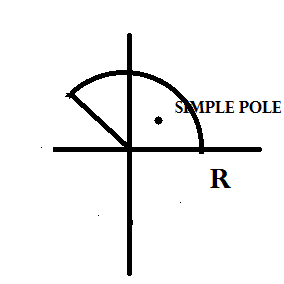
\includegraphics[scale=0.6]{arc.png}
	\end{center}
\end{description}

\subsection{Jordan\rq{}s Inequality}
This inequality will be useful when proving such aforementioned limits tending to zero type identities. The inequality itself is a standard one proven by analysis 
$$\int_{0}^{\pi} \exp(-R\sin\theta) < \frac{\pi}{R}$$ The actual lemma which was originally stated by Jordan is the following. if $f$ is analytic over the semicircle mentioned before and is bounded by some number $\mathcal{M}_{R}$ and if this number tends to zero as R goes to infinity, then for every $a\geq 0$ we have 
$$\lim_{R \to \infty} \int_{\mathcal{C}_{R}} f(z)exp(iaz)dz = 0$$

This is useful in establishing the limiting identity in cases where the integrand involved is a sinusoid. More specifically, if the integrand is a Fourier component, then Jordan\rq{}s lemma comes to the rescue.

\subsection{Argument principle and Rouche\rq{}s Theorem}
We shall deal with \textbf{meromorphic} functions from now on. A function is said to be meromorphic in some domain $\mathcal{D}$ if its singularities consist of poles and only poles. Now, let $f$ be such a meromorphic function and let it traverse a closed Jordan curve $\mathcal{C}$ .  Let it be meromorphic inside the contour, and let it be analytic and nonzero on the contour. Even counting \textbf{multiplicities}. Then, the difference in the argument of $f$ as it traverses one revolution in the contour is a multiple of the difference between the number of zeroes and the number of poles. Mathematically
$$\frac{1}{2\pi}\Delta_{\mathcal{C}} arg f(z) = Z-P$$
This is the famous argument principle. The last theorem of this article concerns with Rouche\rq{}s theorem. The statement: Let $f$ and $g$ be two analytic functions, analytic inside and on a closed contour $\mathcal{C}$. Also let $|f(z)|>|g(z)|$ at each point on $\mathcal{C}$. Then both $f$ and $f+g$\textbf{ have the same number of zeroes, including multiplicities, inside $\mathcal{C}$}.

\subsection{Mittag-Leffler's Theorem}
The theorem is essentially based on expanding meromorphic functions from the poles given in a certain domain of definition. The assumption is that $f(z)$ is analytic at $z=0$, and that the residues at the simple poles $z_1,z_2,z_3,...$ are $b_1,b_2,b_3,...$ respectively. Let the set of poles form a \textbf{modular positively ordered set}. Then,
$$F(z) = f(0) + \sum_{n=1}^\infty b_n(\frac{1}{z-z_n}+\frac{1}{z_n})$$

\subsection{Steepest Descent Technique}
This is a method used to evaluate certain specific type of integrals which generalize a large number of standard integral families like \textit{Bessel, Fourier} etc., and it depends upon the concept of a \textbf{saddle} point and hence is sometimes called as \textbf{saddle point method}. A saddle point is a member of the family of extrema of multivariate functions. Since, the real and imaginary parts of any complex function are in general multivariate functions, we might make a connection here. Given a function $f(x,y)$ we construct the \textbf{Hessian Determinant} $\mathcal{H}$ as follows,
$$\mathcal{H} = f_{xx}(x_0,y_0)f_{yy}(x_0,y_0)-(f_{xy}(x_0,y_0))^2$$
If $\mathcal{H}$ is negative definite, then we say that the point of extremum $(x_0,y_0)$ is a saddle point of $f(x,y)$. With this definition done, we can now dive into the method. It was first found by \textbf{Bernhard Riemann} and is used to evaluate integrals of the form $$I(\lambda) = \int_{\mathcal{C}}e^{\lambda p(z)}q(z)$$ Most of the focus on this method would be on the complex function(polynomial) $p(z)$. If we call $p(z) = u(x,y)+iv(x,y)$, then the integrand is converted to $$e^{\lambda u}e^{i\lambda v}q(z)$$ Now, at large $\lambda$, it is possible to approximate this integral. But, the approximation will only be stable if not for the oscillating factor of $e^{i\lambda v}$. Hence, if $v(x,y) = v(x_0,y_0) = 0$, then one problem has been solved. Therefore, we next look forward to simplifying the utmost structure of $p(z)$ itself. From analysis, we know by experience that polynomials are the most pleasant of all integrable functions to work with. Hence, we need a polynomial expansion of $p(z)$ which is also simplified (we would not like a clumsy Taylor series). We look to expand the function $p(z)$ around one of its saddle points $z_0 = (x_0, y_0)$. In this case, it might become unwieldy to find the real and imaginary parts of $p(z)$, hence, we adopt the following definition of 
\begin{description}
\item[Saddle Points of Order N-1] \hfill \\
	The point $z_0$ is called as the saddle point of order N-1 if $$p'(z_0),p''(z_0),....p^{N-1}(z_0)=0;  p^{N}(z_0) \neq 0$$
\end{description}

Now, expanding in a Taylor series around the saddle point gives us $$p(z) \approx p(z_0)+\frac{(z-z_0)^n}{N!}p^N(z_0)$$
Now, taking the contour to be $z = z_0 + \rho e^{i\theta}$ and that $p^N(z_0) = ae^{i\alpha}$. This substitution leaves us with the following
$$p(z) \approx p(z_0) + \rho^N \frac{ae^{i(N\theta + \alpha)}}{N!}$$
Note that the imaginary or the oscillating part will be zero if and only if $\sin(N\theta+\alpha) = 0$. This implies there are two solutions to $\theta$, one for \textbf{steepest ascent} and the other one for \textbf{steepest descent}. We choose the latter, as the title suggests. Hence, the curve of steepest descent for the function $p(z)$ is given by
$$\theta = -\frac{\alpha}{N} + (2k+1)\frac{\pi}{N}$$
Hence, the algorithm for the method of steepest descent is really just finding the saddle points (according to the last definition) of $p(z)$ and then, using the reduced Taylor expression given above, we can deform the integration contour, checking the consistency with Cauchy's theorem, and we can evaluate the integral using either the contour integration or by simplifying the reduced $e^{p(z)}$ term with standard integrals such as the Gaussian etc.

For more examples on steepest descent technique, refer the notes from 
\url{http://www.maths.manchester.ac.uk/~gajjar/MATH44011/notes/44011_note4.pdf}
\end{sloppypar}
\end{document}